\documentclass[english]{scrartcl}
\usepackage[T1]{fontenc}
\usepackage{listings}
\usepackage{hyperref}
\usepackage{graphicx}
\usepackage{color}
\usepackage{soul}
\usepackage{seqsplit}
\usepackage{multirow}
\usepackage{enumitem}
\usepackage{graphicx}
\usepackage{float}
\usepackage{amsmath}
\begin{document}
\section*{Assignment 7}
\subsection*{Task 7.1}
\begin{enumerate}
\item states:
\\$x_1$ - door1 is reward door, door2 is tiger door, 
\\$x_2$ - door1 is tiger door, door2 is reward door;
\item actions:
\\$u_1$ - open door1 and finish game, terminal action, 
\\$u_2$ - open door2 and finish game, terminal action, 
\\$u_3$ - listen, sensing action, gives measurement $\{z_1, z_2\}$ as result;
\item measurement space:
\\$z_1$ - noise behind the door1,
\\$z_2$ - noise behind the door2;
\item cost function (expected rewards):
\\$r(b,u_1)=p_1*r(x_1,u_1)+p_2*r(x_2,u_1)=p_1*(+200)+(1-p_1)*(-1000)$,
\\$r(b,u_2)=p_1*r(x_1,u_2)+p_2*r(x_2,u_2)=p_1*(-1000)+(1-p_1)*(+200)$,
\\$r(b,u_3)=-50$;
\item associated probabilities:
\\in state $x_1$ person gets $z_1$ with probability 0.2 and $z_2$ with probability 0.8, thus with probability 0.2 he thinks, that tiger is behind the door1 and changes state to $x_2$,
\\in state $x_2$ person gets $z_1$ with probability 0.8 and $z_2$ with probability 0.2, thus with probability 0.2 he thinks, that tiger is behind the door2 and changes state to $x_1$.
\end{enumerate}
Whole scheme is depicted in the Figure \ref{fig:7-1}.

\begin{figure}[h]
\centering
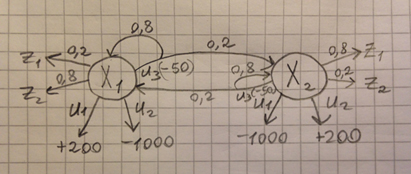
\includegraphics{./7-1}
\caption{POMDP scheme}
\label{fig:7-1}
\end{figure}

\subsection*{Task 7.2}
Cumulative reward (cost) of the sequence "Listen, listen, open door1" is: 
$$R=r(b,u_3)+r(b,u_3)+r(b,u_1)=$$
$$=-50-50+(+200)*p_{1}+(-1000)*(1-p_{1})=-1100-800p_1$$ where $p_1$ is probability of being in $x_1$
\\Person choose action $u_{1}$ anyway, independently of the measurement from $u_{3}$, thus we just sum up doubled cost of doing $u_{3}$ and expected reward after doing $u_{1}$.

\subsection*{Task 7.3}
Cumulative reward (cost) of the sequence "Listen, then open the door for which you did not hear a noise" is:
$$R=r(b,u_3)+=$$
$$=-50+200*0.8-1000*0.2=-90$$
\\Person acts accordingly to the measurement after committing $u_{3}$, thus he opens the door with best measurement with probability 0.8.

\subsection*{Task 7.4}

\end{document}


